\documentclass[a4paper]{article}

\usepackage{INTERSPEECH_v2}

\title{Character Network Extraction from Asimov's Works: \\
A Natural Language Processing Approach}
\name{Martin GERIS$^1$, Evan MASSOL$^2$}
\address{
  $^1$University of Avignon, France\\
  $^2$University of Avignon, France}
\email{martin.geris@alumni.univ-avignon.fr, evan.massol@alumni.univ-avignon.fr}

\begin{document}

\maketitle

\begin{abstract}
This report presents our methodology and results for extracting character networks from Isaac 
Asimov's literary works. Natural Language Processing (NLP) techniques, particularly Named Entity 
Recognition (NER) and relation analysis, were applied to automatically identify characters and their 
interactions. The project addressed key challenges including character alias management, relationship 
extraction, and text preprocessing specific to literary corpus analysis. Results demonstrate the 
effectiveness of combining state-of-the-art NLP tools with domain-specific preprocessing for analyzing 
narrative structures and character dynamics in science fiction literature.
\end{abstract}

\section{Context}

Natural Language Processing (NLP) is a field of computer science and computational linguistics that 
aims to enable machines to understand, analyze, and generate human language. Among its numerous 
applications, extracting character networks from narrative texts constitutes a particular challenge, 
combining Named Entity Recognition (NER) and analysis of relationships between these entities. These 
techniques allow representing character interactions in graph form, providing a powerful tool for 
literary analysis, plot study, and visualization of narrative dynamics.

Within this project, we focused on different corpora from Isaac Asimov's works. The proposed 
challenge consists of automatically extracting characters and identifying their relationships. This 
broad framework reveals numerous complex aspects, particularly related to the narrative and stylistic 
nature of the studied texts.

Several major difficulties were identified from the initial analyses. The first concerns named entity 
recognition. NLP must correctly distinguish characters from other types of entities, such as 
organizations, places, or concepts, which can prove delicate due to ambiguous formulations, honorific 
titles, or compound names. The second difficulty lies in alias management, that is, the different ways 
the same character may be designated in the narrative. The variability of first names, last names or 
nicknames and cases where multiple characters share similar names constitute an additional obstacle to 
automatic extraction.

This report aims to present our methodology and results within this project framework. It details 
the technical choices made for text preprocessing, implementation of character recognition algorithms, 
construction of relationship graphs, and specific adjustments to handle aliases and interactions. The 
objective is also to highlight current limitations of our approach, as well as improvement paths 
identified for future project phases.

For more details and to access the code developed within this project framework, the GitHub 
repository is available at: evan-massol/characters-network-extraction-AMS

\section{State of the Art}

Since the first formal attempts, character network extraction has predominantly relied on a pipeline 
approach, structured in several successive stages: text segmentation into relevant units (chapters), 
detection and normalization of entities corresponding to characters, alias and coreference 
resolution, and finally construction and weighting of the final graph. The foundational work of Elson, 
Dames and McKeown (2010) illustrates this approach, particularly through the use of simple heuristics 
such as character co-occurrence in the same scene or dialogue identification to infer direct interactions.

These heuristic methods have the advantage of being robust and relatively simple to implement, 
particularly on well-structured corpora. However, they rely on the assumption that textual proximity 
reflects a real social relationship, which frequently leads to approximations or artificial relations, 
especially in complex literary texts where narration can be indirect or fragmented.

A major challenge in character network construction lies in reliable recognition of fictional entities. 
This task primarily relies on Named Entity Recognition (NER). Classical approaches, based on 
statistical models or LSTM recurrent neural networks, have shown good performance on journalistic 
texts, but their effectiveness diminishes significantly in the literary context. This limitation is 
explained by the stylistic diversity of works, frequent use of nicknames, periphrases or indirect 
references to characters.

Recent advances are based on the integration of pre-trained Transformer language models, such as 
BERT (Devlin et al., 2019), which allow better context consideration and improve character detection 
in complex narrative texts. Nevertheless, entity recognition alone is insufficient without effective 
coreference resolution. The latter aims to group different linguistic mentions (proper names, pronouns, 
nominal descriptions) referring to the same character. The work of Lee et al. (2017) proposed 
end-to-end neural models for coreference resolution, now widely adopted and adapted to literary 
corpora, as they directly condition the structural coherence of the extracted network.

Once characters are identified and normalized, relation extraction constitutes another central 
problem. The simplest methods rely on co-occurrence in the same textual unit, a widely used but 
limited hypothesis, as it does not distinguish the nature, intensity or direction of relationships. 
More advanced approaches seek to exploit dialogues, communication verbs or syntactic structures to 
extract more semantic relations, such as family, hierarchical or conflictual links.

Recent trends show evolution toward hybrid pipelines that combine robust heuristics and neural 
modules, as well as integration of specialized pre-trained models (BERT, SpanBERT) for NER, 
coreference and relation extraction. Sims and Bamman (2020) notably propose methods exploiting graphs 
to model information propagation and temporal dynamics of character interactions. Furthermore, the 
emergence of Graph Neural Networks opens new perspectives to refine the final relational structure and 
capture network evolution throughout the narrative.

In summary, automatic character network extraction is a complex task, requiring the integration of 
several NLP subtasks. Despite significant advances, particularly thanks to pre-trained language 
models, many challenges persist, fully justifying current research and the development of new systems 
better adapted to the specificities of literary texts.

\section{NLP Tools}

NLP tools are based on complex architectures, most often founded on deep neural networks requiring 
significant volumes of training data. The design and training of such models constitute considerable 
work that could alone justify a complete research project. However, given the objectives pursued in 
this project, it appeared more relevant to reuse existing libraries rather than develop specific 
algorithms.

In this perspective, we compared two libraries recognized for their performance, offering a complete 
processing chain from tokenization (extraction of textual units like words or punctuation) to named 
entity recognition (NER). To evaluate the effectiveness of spaCy (Explosion AI, 2024) and Stanza 
(Qi et al., 2020), we developed a short story of about ten lines, integrating direct and indirect 
dialogues. This text was then processed independently by each of the two libraries. The obtained 
results are presented in part in Figure 1 and analyzed below.

The analysis reveals generally more precise tokenization with spaCy. Conversely, Stanza tends to 
group multiple textual elements within the same token, generating notable errors. These imprecisions 
seem mainly linked to imperfect punctuation handling. Differences also appear in character 
recognition: for example, spaCy classifies the expression "minister of Health" as an organization 
rather than as a character. While this error is debatable, it remains marginal compared to the 
tokenization problems observed with Stanza. Thus, spaCy proved more adapted to this project's needs 
and was retained for subsequent work.

\begin{figure}[ht]
    \centering
    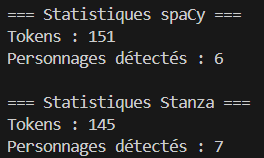
\includegraphics[width=0.45\textwidth]{figures/spacy_stanza_comparison.png}
    \caption{Comparison of tokenization and named entity recognition results between spaCy (top) 
    and Stanza (bottom) on a short story.}
    \label{fig:spacy_stanza_comparison}
\end{figure}

On reduced-size corpora, the spaCy library proves particularly performant and generates few 
manifestly inconsistent errors, such as identifying a verb as a character. Nevertheless, when 
processing longer texts — particularly within Isaac Asimov's corpora — certain anomalies appear. 
To limit these errors, a text preprocessing step proves indispensable; it will be detailed 
subsequently. However, this preprocessing is not always sufficient alone.

This is where anti-dictionaries come into play. These are lists of terms explicitly excluded from 
recognition as characters. These dictionaries are progressively enriched during program development, 
as new errors are identified. Nevertheless, their use must remain measured and targeted, as nothing 
guarantees that an author adopts classical naming conventions for their characters. Isaac Asimov 
provides an emblematic example by naming one of his characters "Dors," a term that, out of context, 
could be interpreted as a common noun.

\section{Text Preprocessing}

In his works, Isaac Asimov employs particular linguistic processes, such as the intentional use of 
truncated words, to immerse the reader in the atmosphere of ancient manuscripts or incomplete 
narratives. While these stylistic choices enrich the narrative dimension, they constitute a 
significant obstacle for automatic text analysis. Added to these specificities are other 
difficulties that complicate automatic natural language processing. These notably include the 
presence of elements external to the narrative — such as page numbers —, characters misinterpreted 
during extraction, or the systematic absence of every other page due to copyright constraints.

In this context, it appears indispensable to rework the initial textual material to obtain a more 
homogeneous corpus, approaching standard language and thus more easily exploitable by NLP tools. To 
address this challenge, a preprocessing step was integrated into our pipeline. This aims to remove or 
transform identified problematic elements, with the objective of guaranteeing the most reliable 
subsequent processing possible.

The .pdf format files at our disposal must first be converted to .txt files. This operation 
nevertheless preserves various parasitic elements, such as page numbers, section titles, and chapter 
headings. These can be removed effectively using regular expressions (regex).

A particularly determining aspect of preprocessing concerns the structure of the provided corpora 
themselves, which contain only every other page. This constraint causes fragmentation of certain 
sentences that find themselves deprived of their beginning, others of their ending. These incomplete 
textual segments, often lacking subject or verb, are difficult to analyze automatically and can alter 
result quality. Therefore, a methodological choice is imposed: should we preserve these truncated 
sentences to preserve maximum data, or on the contrary remove them to exclude lower-quality text 
portions? Given our still limited mastery of NLP tools, we opted, at this project stage, for 
removing these fragments.

Currently, only one of the provided corpora has undergone complete preprocessing: the Foundation 
corpus. Each corpus indeed seems to follow its own logic, both in page organization and in regular 
expressions necessary for identifying numbers, chapters, or sections. It will therefore be necessary 
to adapt preprocessing scripts to each of the studied corpora.

Finally, preprocessing appears as crucial a step as natural language processing itself, insofar as 
the latter cannot be conducted effectively without adequate data preparation. Its improvement is thus 
part of an iterative approach, evolving jointly with advances made in NLP methods.

\section{Alias Management}

In a narrative, the same character can be designated in multiple ways; these different appellations 
are commonly grouped under the term alias. Identifying these appellations and the characters to which 
they are linked constitutes one of the major challenges of automatic character network extraction 
from narrative texts. At this stage of our experiments, it appeared that the spaCy library did not 
offer a satisfactory solution for managing these aliases. To compensate for this limitation, we 
developed specific algorithms dedicated to their handling.

Within our pipeline, we construct a dictionary named aliases\_map, in which each key corresponds 
to an identified character, and each value to one of their aliases. In the current state of our 
implementation, only so-called "obvious" aliases are considered, namely those corresponding 
exclusively to the character's family name, first name, or combination of both.

This voluntarily simplified approach presents limitations and will need future enrichment. 
Indeed, several complex cases are not yet covered: the presence of characters sharing 
the same first name or same last name, situations where a character possesses multiple first names 
or multiple last names, as well as aliases not based on usual anthroponyms. These configurations, 
frequent in literary works, will require more advanced disambiguation strategies.

\section{Relationship Management}

The second major objective of character network extraction lies in identifying relationships between 
different entities. This task proves just as complex as character identification itself. Nevertheless, 
the guidelines defined within the project framework allow simplifying the approach. Indeed, these 
establish that a relationship is determined solely by the proximity of two named entities within the 
narrative. More precisely, two characters are considered to be in relationship as soon as one of 
their respective occurrences in the corpus is separated by 25 tokens or fewer. While this heuristic 
rule may be disputed in certain situations — particularly when textual proximity does not reflect 
real narrative interaction — it constitutes an acceptable compromise within this work framework.

To model relationships between identified characters, we construct, within our pipeline, a dictionary 
entitled relations\_map. In this structure, each key corresponds to a character pair, while the 
associated value represents the number of relationship identification occurrences involving them.

\section{Results}

During the major part of the time devoted to this project, our work mainly focused on the corpora 
used for the leaderboard. This focus allowed us to obtain the results presented in Figure 2. Analysis 
of this visualization shows that the more an entity is distant from the graph center, the more reduced 
the number of chapters in which it appears. Inversely, the most central characters correspond to those 
whose presence is most recurrent in the narrative. Unsurprisingly, the work's main protagonist, 
Harry Seldon, occupies the central position of the graph. On the contrary to what was initially 
expected, the edges don't reflect the number of co-occurrences between characters, but rather the number 
of relationships identified according to the amount of times two characters are found within a same
chapter. This is bound to change in future versions of the project.

\begin{figure}[ht]
    \centering
    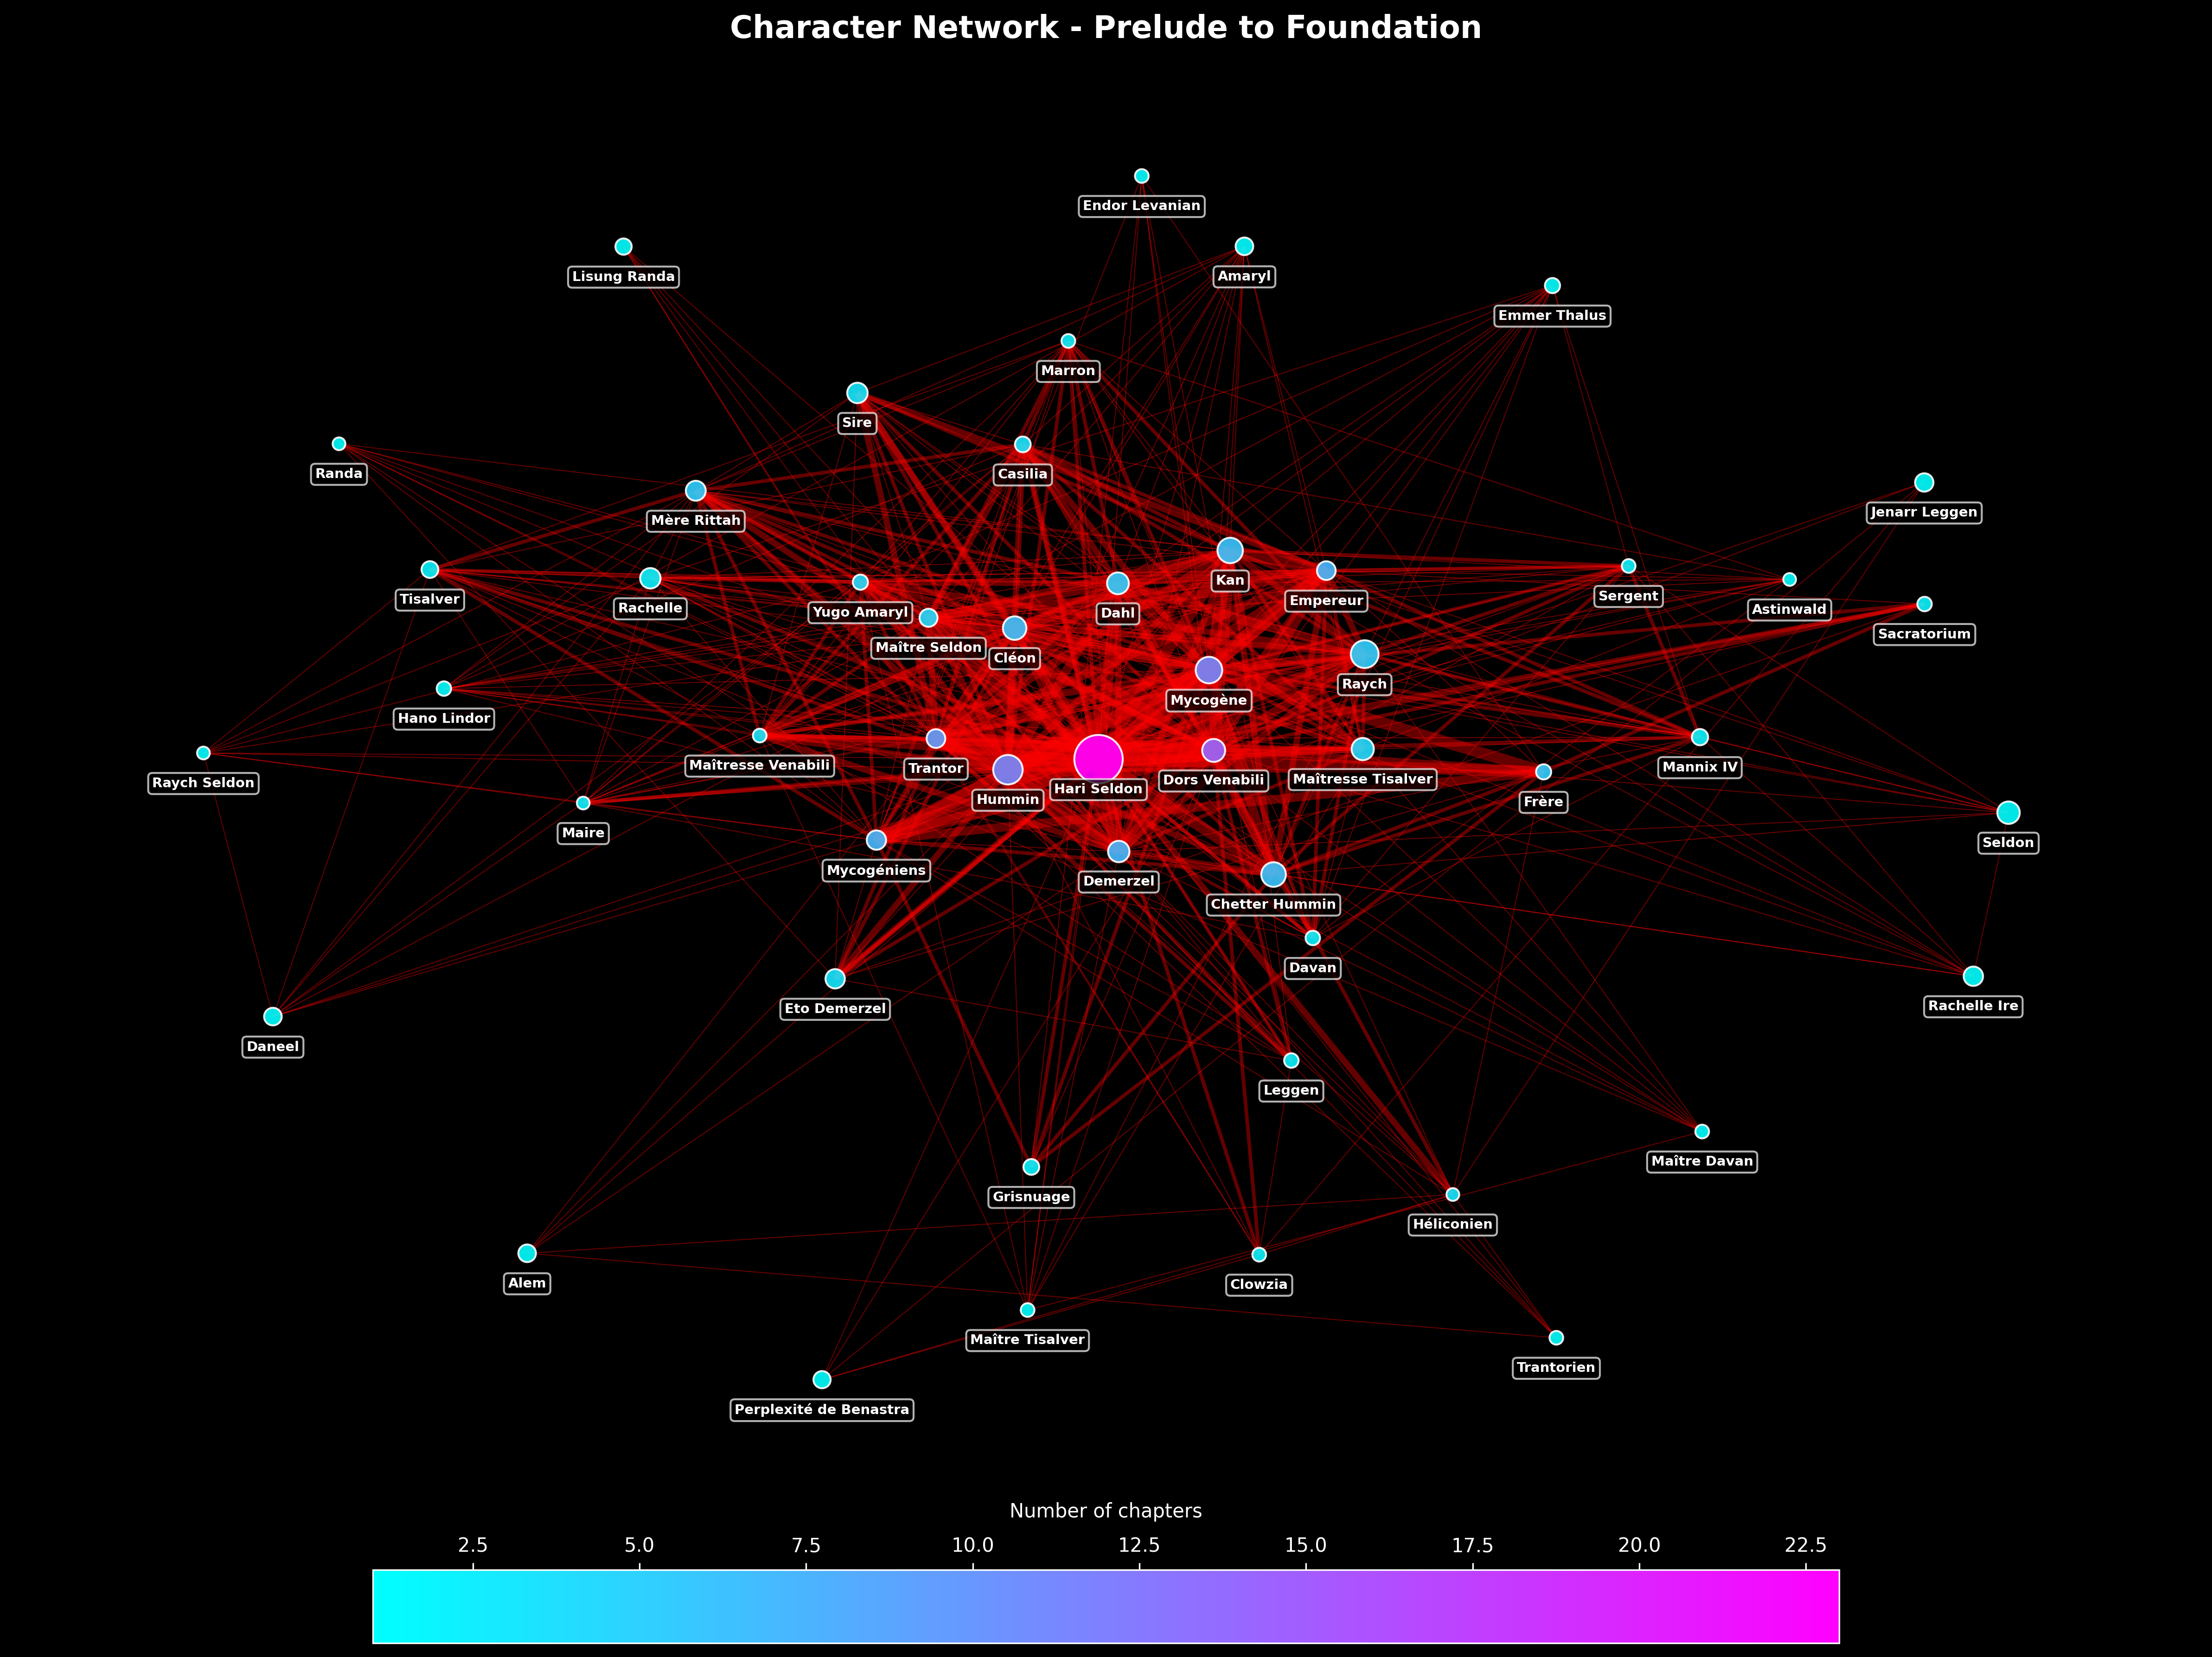
\includegraphics[width=0.45\textwidth]{figures/foundation_graph.png}
    \caption{Character network extracted from the Foundation corpus. Node size reflects the 
    number of chapters in which the character appears; edge thickness indicates the number of identified 
    relationships between characters.}
    \label{fig:foundation_graph}
\end{figure}

\section{Improvement Directions}

The project is still only in its beginnings and numerous improvements can be brought to it in the 
future. In this section, we review each major step presented previously and discuss possible 
improvement paths.

\subsection{Preprocessing}

To date, certain problems identified previously have not yet been addressed. For example, we have not 
yet tackled processing expressions voluntarily truncated by the author. Nevertheless, we think it 
would be possible, using an appropriate library, to attempt reconstructing these truncated words 
based on the few available letters and their position in the word.

We also observed that certain manifest NLP errors can be attributed to the imperative structure of 
certain sentences, direct discourse, or use of particular characters such as dashes. No solution has 
yet been implemented to correct these cases. Several approaches are conceivable. The simplest solution 
would consist of removing these problematic segments. However, more sophisticated treatments, allowing 
preservation of narrative content from concerned excerpts, would be preferable. For example, for 
imperative sentences, it might be useful to add a subject to facilitate their automatic analysis.

\subsection{Alias Management}

Alias management seems to us the most dizzying challenge of this project. According to our research, 
solutions proposed in the literature show that no isolated strategy allows satisfactorily resolving 
all alias phenomena in narrative context. The most robust approaches generally rely on a combination 
of linguistic rules, contextual disambiguation, and constraints derived from the character network 
structure itself. In this perspective, our work is inscribed as a first voluntarily simplified step, 
opening the way to progressive integration of these more advanced methods using appropriate libraries.

\subsection{Relationship Management}

Given the guidelines simplifying the approach to this problem, we do not judge it necessary to 
deeply rework our existing algorithms, beyond some minor logical adjustments. On the other hand, 
evaluating the nature of relationships between characters seems to constitute a relatively accessible 
evolution perspective.

In a narrative, relationships between characters can take various forms — romantic, familial, 
professional, among others. By reducing this diversity to a unidimensional scale ranging from friendly 
relationship to hostile relationship, it would become possible to represent these interactions 
synthetically within produced graphs.

To study this dimension, we envision identifying semantic values associated with words appearing in 
the textual interval defining a relationship using an appropriate library. The studied interval will 
constitute the text portion between occurrences of the first and second character. If this approach 
proved insufficient, it might also be relevant to extend analysis to terms located in immediate 
proximity to citations of concerned characters, introducing a parameter defining an analysis radius 
around occurrences.

\section{Conclusion}

This project enabled exploring and implementing a pipeline for automatic character network extraction 
from narrative texts, based on corpora from Isaac Asimov's works. We presented key steps, from text 
preprocessing to relationship graph construction, through named entity recognition, alias management, 
and identification of character interactions.

Our results show that the chosen approach, combining use of performant libraries such as spaCy with 
specific treatments adapted to literary corpora, allows obtaining coherent graphs in which main 
characters and their interactions are correctly highlighted. Conducted analyses confirm the importance 
of preprocessing and textual data normalization, as well as the crucial role of alias management for 
ensuring reliability of extracted networks.

However, this work still constitutes a first step. Numerous limitations persist, particularly in 
managing complex aliases, reconstructing truncated words, semantic analysis of relationships, and 
considering fragmented or atypical sentences. These challenges open interesting perspectives for 
future project evolutions, such as contextual analysis of relationships.

\begin{thebibliography}{9}

\bibitem{devlin2019}
Devlin, J., Chang, M.-W., Lee, K., \& Toutanova, K. (2019). BERT: Pre-training of deep 
bidirectional transformers for language understanding. Proceedings of NAACL-HLT 2019.

\bibitem{elson2010}
Elson, D. K., Dames, N., \& McKeown, K. R. (2010). Extracting social networks from literary fiction. Proceedings of the 48th Annual Meeting of the Association for Computational Linguistics.

\bibitem{spacy2024}
Explosion AI. (2024). spaCy (version 3.7) [Software]. https://spacy.io

\bibitem{labatut2019}
Labatut, V., \& Bost, X. (2019). Extraction and analysis of fictional character networks: A survey. arXiv:1907.02704.

\bibitem{lee2017}
Lee, K., He, L., Lewis, M., \& Zettlemoyer, L. (2017). End-to-end neural coreference resolution. Proceedings of EMNLP 2017.

\bibitem{stanza2020}
Qi, P., Zhang, Y., Zhang, Y., Bolton, J., \& Manning, C. D. (2020). Stanza (version 1.6) 
[Software]. https://stanfordnlp.github.io/stanza/

\bibitem{sims2020}
Sims, M., \& Bamman, D. (2020). Measuring information propagation in literary social networks. Proceedings of ACL 2020.

\end{thebibliography}

\end{document}
